\section{The basics}
Models are constructed from building blocks which have been created in \CPP\ using the \US\ programming framework. For your first models you should use the pre-existing building blocks which are included with your \US\ installation. Only later on you might want to create your own building blocks in \CPP.

To build a model, you put building blocks together in a \concept{box script} which is a text file written according to a few rules. In the box script, you declare which building blocks your model consists of, how they are organised, and how they interact. The box script language is an example of a domain-specific programming language \citep{HolstBelete}.

When you work with a model, you go through these steps again and again:

\begin{enumerate}
\item Launch the software (\US, R and text editor).
\item In \US, run the box script that defines your model.
\item In R, view the model output.
\item \label{NielsH} In the text editor, make any desired changes to the box script, save, and go back to step 2.
\end{enumerate}

The box script found in \filenameexplained{book/egg1.box} is a good starting point. To get started, issue the \code{load} command and then the \code{edit} command at the \US\ prompt. Like this:

\lstset{numbers=left}
\begin{usdialog}
> load book/egg1.box
Construct...
Amend...
6 boxes created
> edit
\end{usdialog}
\lstset{numbers=none}

For a start we won't run the box script, only load it into \US. That is why we used the \code{load} command in line 1 rather than the \code{run} command. The \code{edit} command will open the box script in the text editor:

\lstset{numbers=left}
\begin{boxscript}
// egg1.box
Simulation sim {
  .steps = 14
  Stage egg {
    .initial = 100 
    .duration = 7
  }
  OutputR {
    PageR {
      .width = 4
      .height = 2.5
      .xAxis = sim[step]
      PlotR {
        .ports = egg[content]
      }
    }
  }
}
\end{boxscript}
\lstset{numbers=none}

In plain language, \filename{egg1.box} contains a simulation model (line 2) which will run in 14 steps (line 3). It contains an \code{egg} stage (line 4) with an initial number of 100 eggs (line 5) and an average duration of 7 time steps (line 6). The output will go to R (line 8), which will produce a page (line 9) of the given dimensions (lines 10-11) using the simulation time step for the \xaxis\ (line 12). The page contains one plot (line 13) with the number of eggs on the \yaxis\ (line 14). The dimensions are in inches and were chosen to produce a figure suitable for this book. The dimensions are ignored if you use R Studio. Only in the classic R GUI will they have an effect.

We would expect the output to show a declining curve as the eggs hatch. Type \code{run} and then paste the clipboard into R. You should get the result shown in \iref{fig:egg1}.

\begin{figure} [b]
\centering
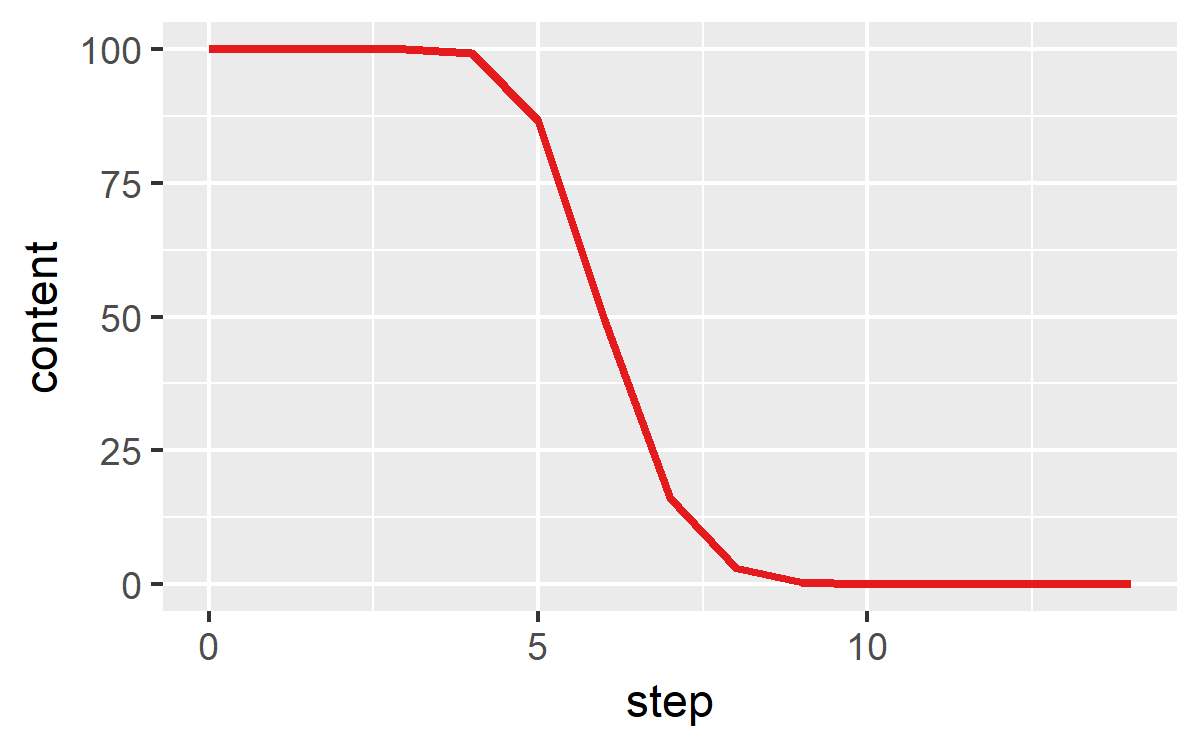
\includegraphics{graphics/egg1}
\caption{Egg hatching curve generated by \filename{\inputfolder/book/egg1.box}.}
\label{fig:egg1}
\end{figure}

In the \filename{egg1.box} script, we find examples of five \concept{building blocks} (\code{Simulation, Stage, OutputR, PageR, PlotR}). More precisely, these are different \concept{Box classes} defined in the \CPP\ source code. Taken together, all the \code{Box} classes available for \US\ form a toolbox of building blocks with which to build models. 

The toolbox is organised into modules (or plug-ins) each with a selection of \code{Box}'es. To see all the \code{Box}'es available in the \code{boxes} module (thus named, because this is the standard module), type this at the prompt:

\begin{usdialog}
> help boxes
\end{usdialog}

To get the details of a particular \code{Box}, type \eg,
\begin{usdialog}
> help Sun
\end{usdialog}

You will later learn how to add your own module with your own \code{Box} classes to the toolbox (\iref{ch:basic-cpp}).

Whenever a \code{Box} \concept{class} is used in a box script, a \code{Box} \concept{object} is created in your computer's memory. In this box script we explicitly created five objects, one of each class. Two of them have names to identify them: \code{sim} and \code{egg}, while the other three remain unnamed. 

Some \code{Box} objects may create additional \code{Box} objects. In this case, one additional \code{Box} was created by the \code{OutputR} box. This is why \US\ reported '6 boxes created' in line 4 of the dialog above.

You can get a quick overview of all current \code{Box} objects by the \code{list} command (\iref{commands:list}). Thus you will find that an additional \code{Box} object of the \code{OutputText} class was created inside the \code{OutputR} box:

\lstset{numbers=left}
\begin{usdialog}
> list
Simulation sim
  Stage egg
  OutputR 
    PageR 
      PlotR 
    OutputText 
>
\end{usdialog}
\lstset{numbers=none}

When we speak loosely of a \concept{box}, we might be thinking of either  a box class or a box object. Likewise, we may talk of a \concept{model} rather than a box, in the many cases where the box in fact implements a model, or rather, a \concept{sub-model} since we construct models out of other models. When you develop a new box class (in \CPP), it is difficult to tell how it will be used. Will it be a sub-model, a sub-sub-model, or what? In the \filename{egg1.box} script we would call both \code{sim} and \code{egg} models; \code{sim} is a complex model (a box object containing four other box objects), and \code{egg} is a simple model (a box object containing no other box objects). We use this flexibility of language not to be inconcise put to focus on the essence: An egg model remains an egg model, no matter how many sub-models, it might contain. If we improve the egg model later on, adding more sub-models, we can keep thinking about it simply as the 'egg model'.

The box objects are arranged in a hierarchy, like Chinese boxes, with \code{sim} being the outermost. Alternatively, you can think of the structure as a tree with \code{sim} at the root:

\medskip
\tikzstyle{every node}=[draw=black,anchor=west]
\begin{tikzpicture}[%
  grow via three points={one child at (0.5,-0.7) and
  two children at (0.5,-0.7) and (0.5,-1.4)},
  edge from parent path={(\tikzparentnode.south) |- (\tikzchildnode.west)}]
  \node {Simulation sim}
   child {node {Stage egg}}
   child {node {OutputR}
     child {node {PageR}
       child {node {PlotR}}
     }
     child [missing] {}
     child {node {OutputText}}
   }
  ;
\end{tikzpicture}

\bigskip
In a box script, such as \filename{egg1.box}, names with a leading dot are examples of \concept{input ports} (\code{.steps, .initial, .duration, .xAxis, .ports}). Note that we write the leading dot in front of a port name, only when we set its value. If we choose not set the value of an input port in the box script, it will retain its default value defined in the \CPP\ source code.

The first five ports mentioned in \filename{egg1.box} (lines 3, 5-6, 10-11) are set to fixed values while the last two (lines 12 and 14) \concept{refer} to other ports. We also say that they \concept{import} another port. This means that their value will vary during the simulation, as they track the value of the ports they refer to. 

Ports are referred to by way of path expressions (\iref{ch:path-expressions}). In these two cases, the path simply defines the name of a box object and (in brackets) one of its ports. To write paths like these, you need to know which input and output ports are available for different boxes. You can use the \code{help} command (\iref{commands:help}) to see all the input and output ports available for a class.

You can set an input port equal to another input or output port. However, you can never in a box script set the value of an output port. Output ports are governed strictly by their \CPP\ implementation. For brevity we may call input ports simply \concept{inputs} and output ports, simply \concept{outputs}.

As the port name \code{ports} of the \code{PlotR} class suggests, this input port accepts more than one input. We supply this on vector form, simply by separating elements with spaces and embracing the whole vector with parentheses. Here, we have changed the value of \code{ports} to take two inputs. By default plots inside a page will be stacked. Here we have set the \code{ncol} input to 2 to set the plots side by side:

\lstset{numbers=left}
\begin{boxscript}
// egg2.box
Simulation sim {
:
:
  OutputR {
    PageR {
:
:
      PlotR {
        .ports = (egg[content] egg[outflowTotal])
        .ncol = 2
      }
    }
  }
}
\end{boxscript}
\lstset{numbers=none}

You can try to make this change to \filename{egg1.box} in the text editor yourself. Begin with step 4 on page \pageref{NielsH} and then follow up with steps 2 and 3. Alternatively, you can load the \filename{egg2.box} script. You should get the simulation output seen in \iref{fig:egg2}.
 
\begin{figure}
\centering
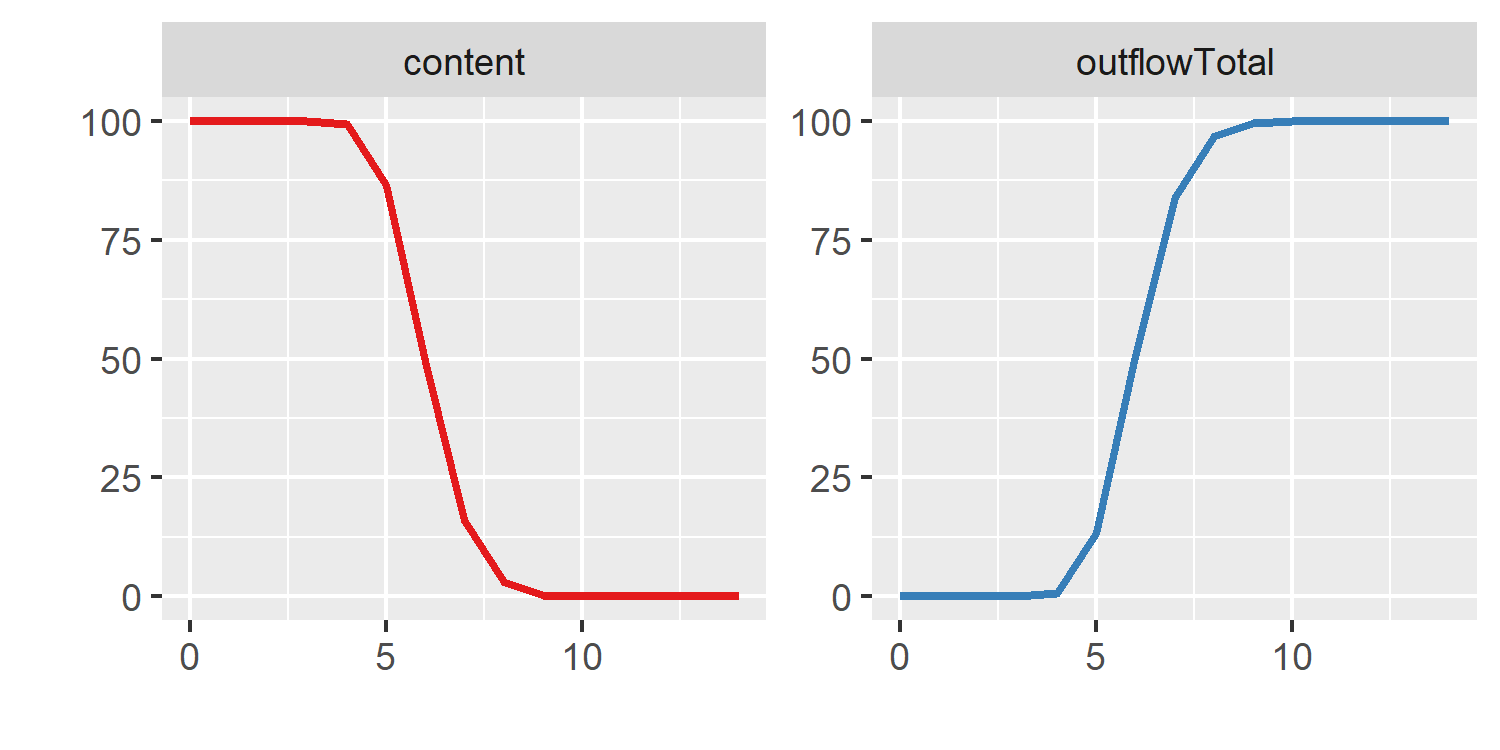
\includegraphics{graphics/egg2}
\caption{Egg hatching curves generated by \filename{\inputfolder/book/egg2.box}.}
\label{fig:egg2}
\end{figure}

The style of your box script coding will be revealing. An experienced (or orderly born) programmer will keep the code neat with whitespace (tabs and blanks) in place to indicate the logical structure, and a few comments for clarification. Comments in box scripts begin with \code{//} and run to the end of the line (as in line 1 above).

Note that, for convenience, you should keep the three programs (\US, R and text editor) open always. Just remember to save the box script after changing it in the text editor, before loading it in \US. Otherwise, any changes carried out in the text editor will go unnoticed in \US. To be cautious, save the box script under another name before changing it. That way, you can always return to an earlier, working version.

\section{Time and weather}
We were not clear about the exact time scale in the egg model. In the next version, we make use of the \code{Calendar} class to keep track of time explicitly:

\lstset{numbers=left}
\begin{boxscript}
// egg3.box
Simulation sim {
  .steps = 14
  Calendar calendar {
    .timeStep = 1
    .timeUnit = "d"
    .initialDateTime = 1/5/2009
  }
  Stage egg {
    .initial = 100 
    .duration = 7
  }
  OutputR {
:
:
  }
}
\end{boxscript}
\lstset{numbers=none}

There are no interactions between the two models \code{calendar} and \code{egg}; they are ignorant of each other. However, the output now shows date on the \xaxis\ and makes clear that the period of simulation spans the first two weeks of May (\iref{fig:egg3}). This has been set up by the \code{Calendar} inputs: \code{timeStep}, \code{timeUnit} and \code{initialDate} (lines 5-7). 

\begin{figure}
\centering
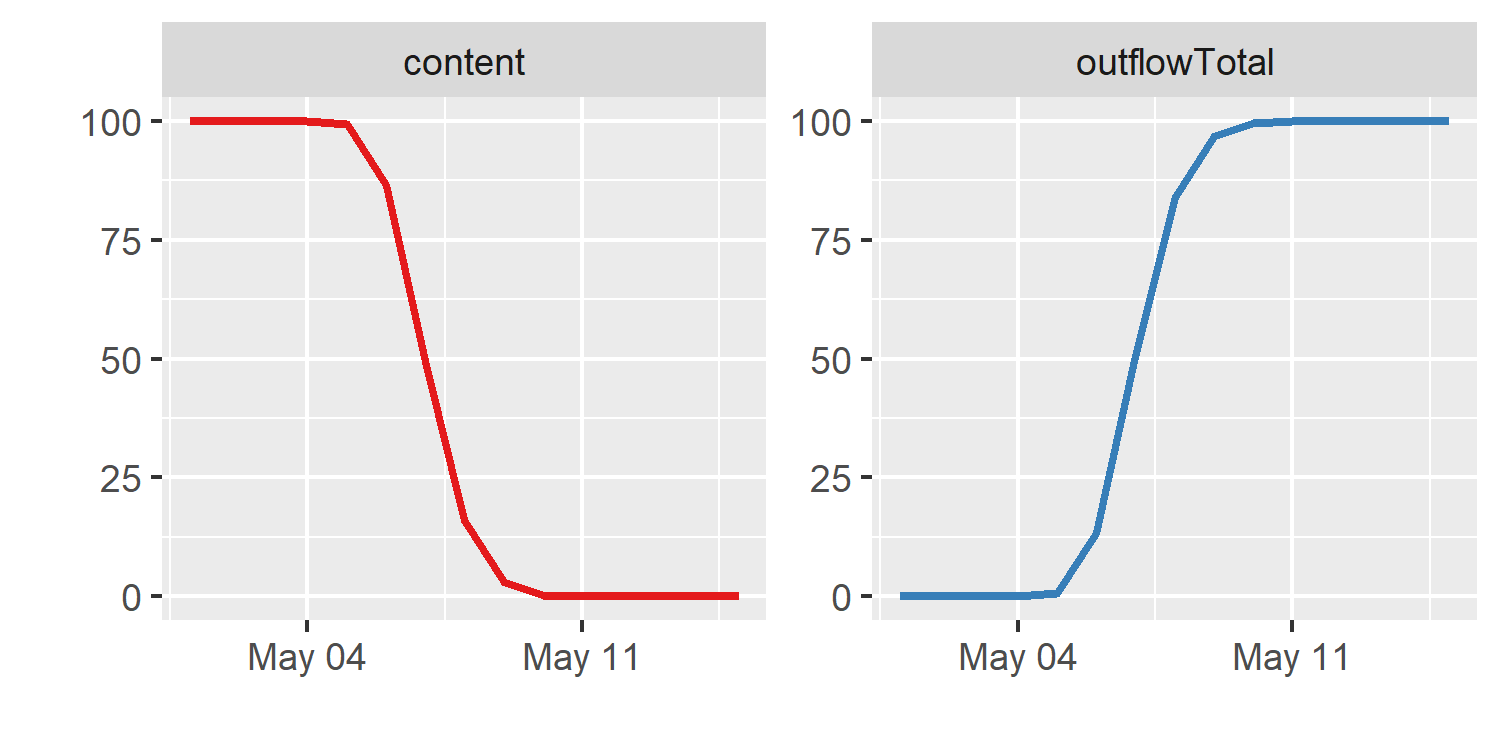
\includegraphics{graphics/egg3}
\caption{Egg hatching curves on a calendar scale. Generated by \filename{\inputfolder/book/egg3.box}.}
\label{fig:egg3}
\end{figure}

The \code{Calendar} class has many ports, both input and output. Type \uscom{help Calendar} at the \US\ prompt to see them (\iref{commands:help}). We note that \code{timeStep} takes an integer number. The time unit is given as a separate input of one character (\code{timeUnit}). The apostrophes tell that \code{"d"} is not a  reference to another port but a simple text. The first date of the calendar (\code{initialDateTime}) is given here in \textit{day/month/year} format. See \iref{ch:type-dates-times} for date and time formats in general.

Let's say that the eggs are not of a bird but of a butterfly. In that case, development time would depend on ambient temperature. Temperature-dependent development is often modelled by the day-degree model. To apply that, we need first to provide our model with weather data.

We can use a \code{Records} box to read weather data supplied as a text file. The text file must be formatted in the style of an R data frame, \ie\ as a file with column headers and a row for each record, as in a weather log. Here are the first three lines of one of the included weather files (\filename{\inputfolder/book/weather/flakkebjerg 2009.txt}):

\lstset{tabsize=8}
\begin{boxscript}
Station  Date    Tmin  Tmax  Tavg  I
6135  01/01/2009  0.5  0.9  2.6  3.2
6135  02/01/2009  -5.4  0.6  -2.8  3.2
6135  03/01/2009  -5.2  3.5  1.2  0.8
\end{boxscript}
\lstset{tabsize=2}

In this particular file, the columns specify the weather station number, the date, daily minimum, maximum and average temperature (\si{\degreeCelsius}), and solar irradiation (\si{MJ/m^2/d}). An input file for \code{Records} must have one column (named \code{Date}), or two columns (named \code{Date} and \code{Time}), to indidate the time stamp of each line. See \iref{ch:type-dates-times} for the various accepted date and time formats. 

If you are not satisfied with the default names \code{Date} and \code{Time} for the date and time columns in the weather file, you can change their names through the \code{dateColumnName} and \code{timeColumnName} inputs to \code{Records}. See \code{help Records}.

For each column in the input file, \code{Records} will create one output port identified by the name of the column heading.

Missing values are not allowed in the columns but if rows are left out, the \code{Records} box will automatically interpolate (linearly) the missing rows. If you run the model on a time step shorter than that of the weather file, values will be interpolated likewise (\eg\ if you set the time step in \code{calendar} to 1 hour with a weather file containing daily records).

Here, we have extended the \filename{egg3.box} script further with a \code{Records} model called \code{weather}. Recall that \code{Records} is the class name and \code{weather} is the object name:

\lstset{numbers=left}
\begin{boxscript}
// egg4.box
Simulation sim {
  .steps = 14
  Calendar calendar {
    .timeStep = 1
    .timeUnit = "d"
    .initialDateTime = 1/5/2009
  }
  Records weather {
    .fileName = "weather/flakkebjerg 2009.txt"
  }
  Stage egg {
    .initial = 100 
    .duration = 7
  }
  OutputR {
    PageR {
:
:
    .xAxis = calendar[date]
      PlotR {
        .ports = (egg[content] egg[outflowTotal])   
        .ncol = 2
      }
      PlotR {
        .ports = weather[Tavg]   
      }
    }
  }
}
\end{boxscript}
\lstset{numbers=none}

The \code{Records} box takes a \code{fileName} as input (line 10). This could be a bare file name (\ie\ a file name without a path), or it could include a relative path. In this case, \code{fileName} denotes a file named \filename{flakkebjerg 2009.txt} in a folder named \filename{weather} (\ie, \filename{weather} is the relative path). 

The \code{Records} box will seach for the given \code{fileName} first in the same folder as the box script (here \filename{\inputfolder/book}), then it will look in the parent folder, and then further upwards in the folder hierarchy. In this case, it will succeed finding the file: \filename{\inputfolder/book/weather/flakkebjerg 2009.txt}. You should check for yourself that you can indeed locate the file there.

\begin{figure} 
\centering
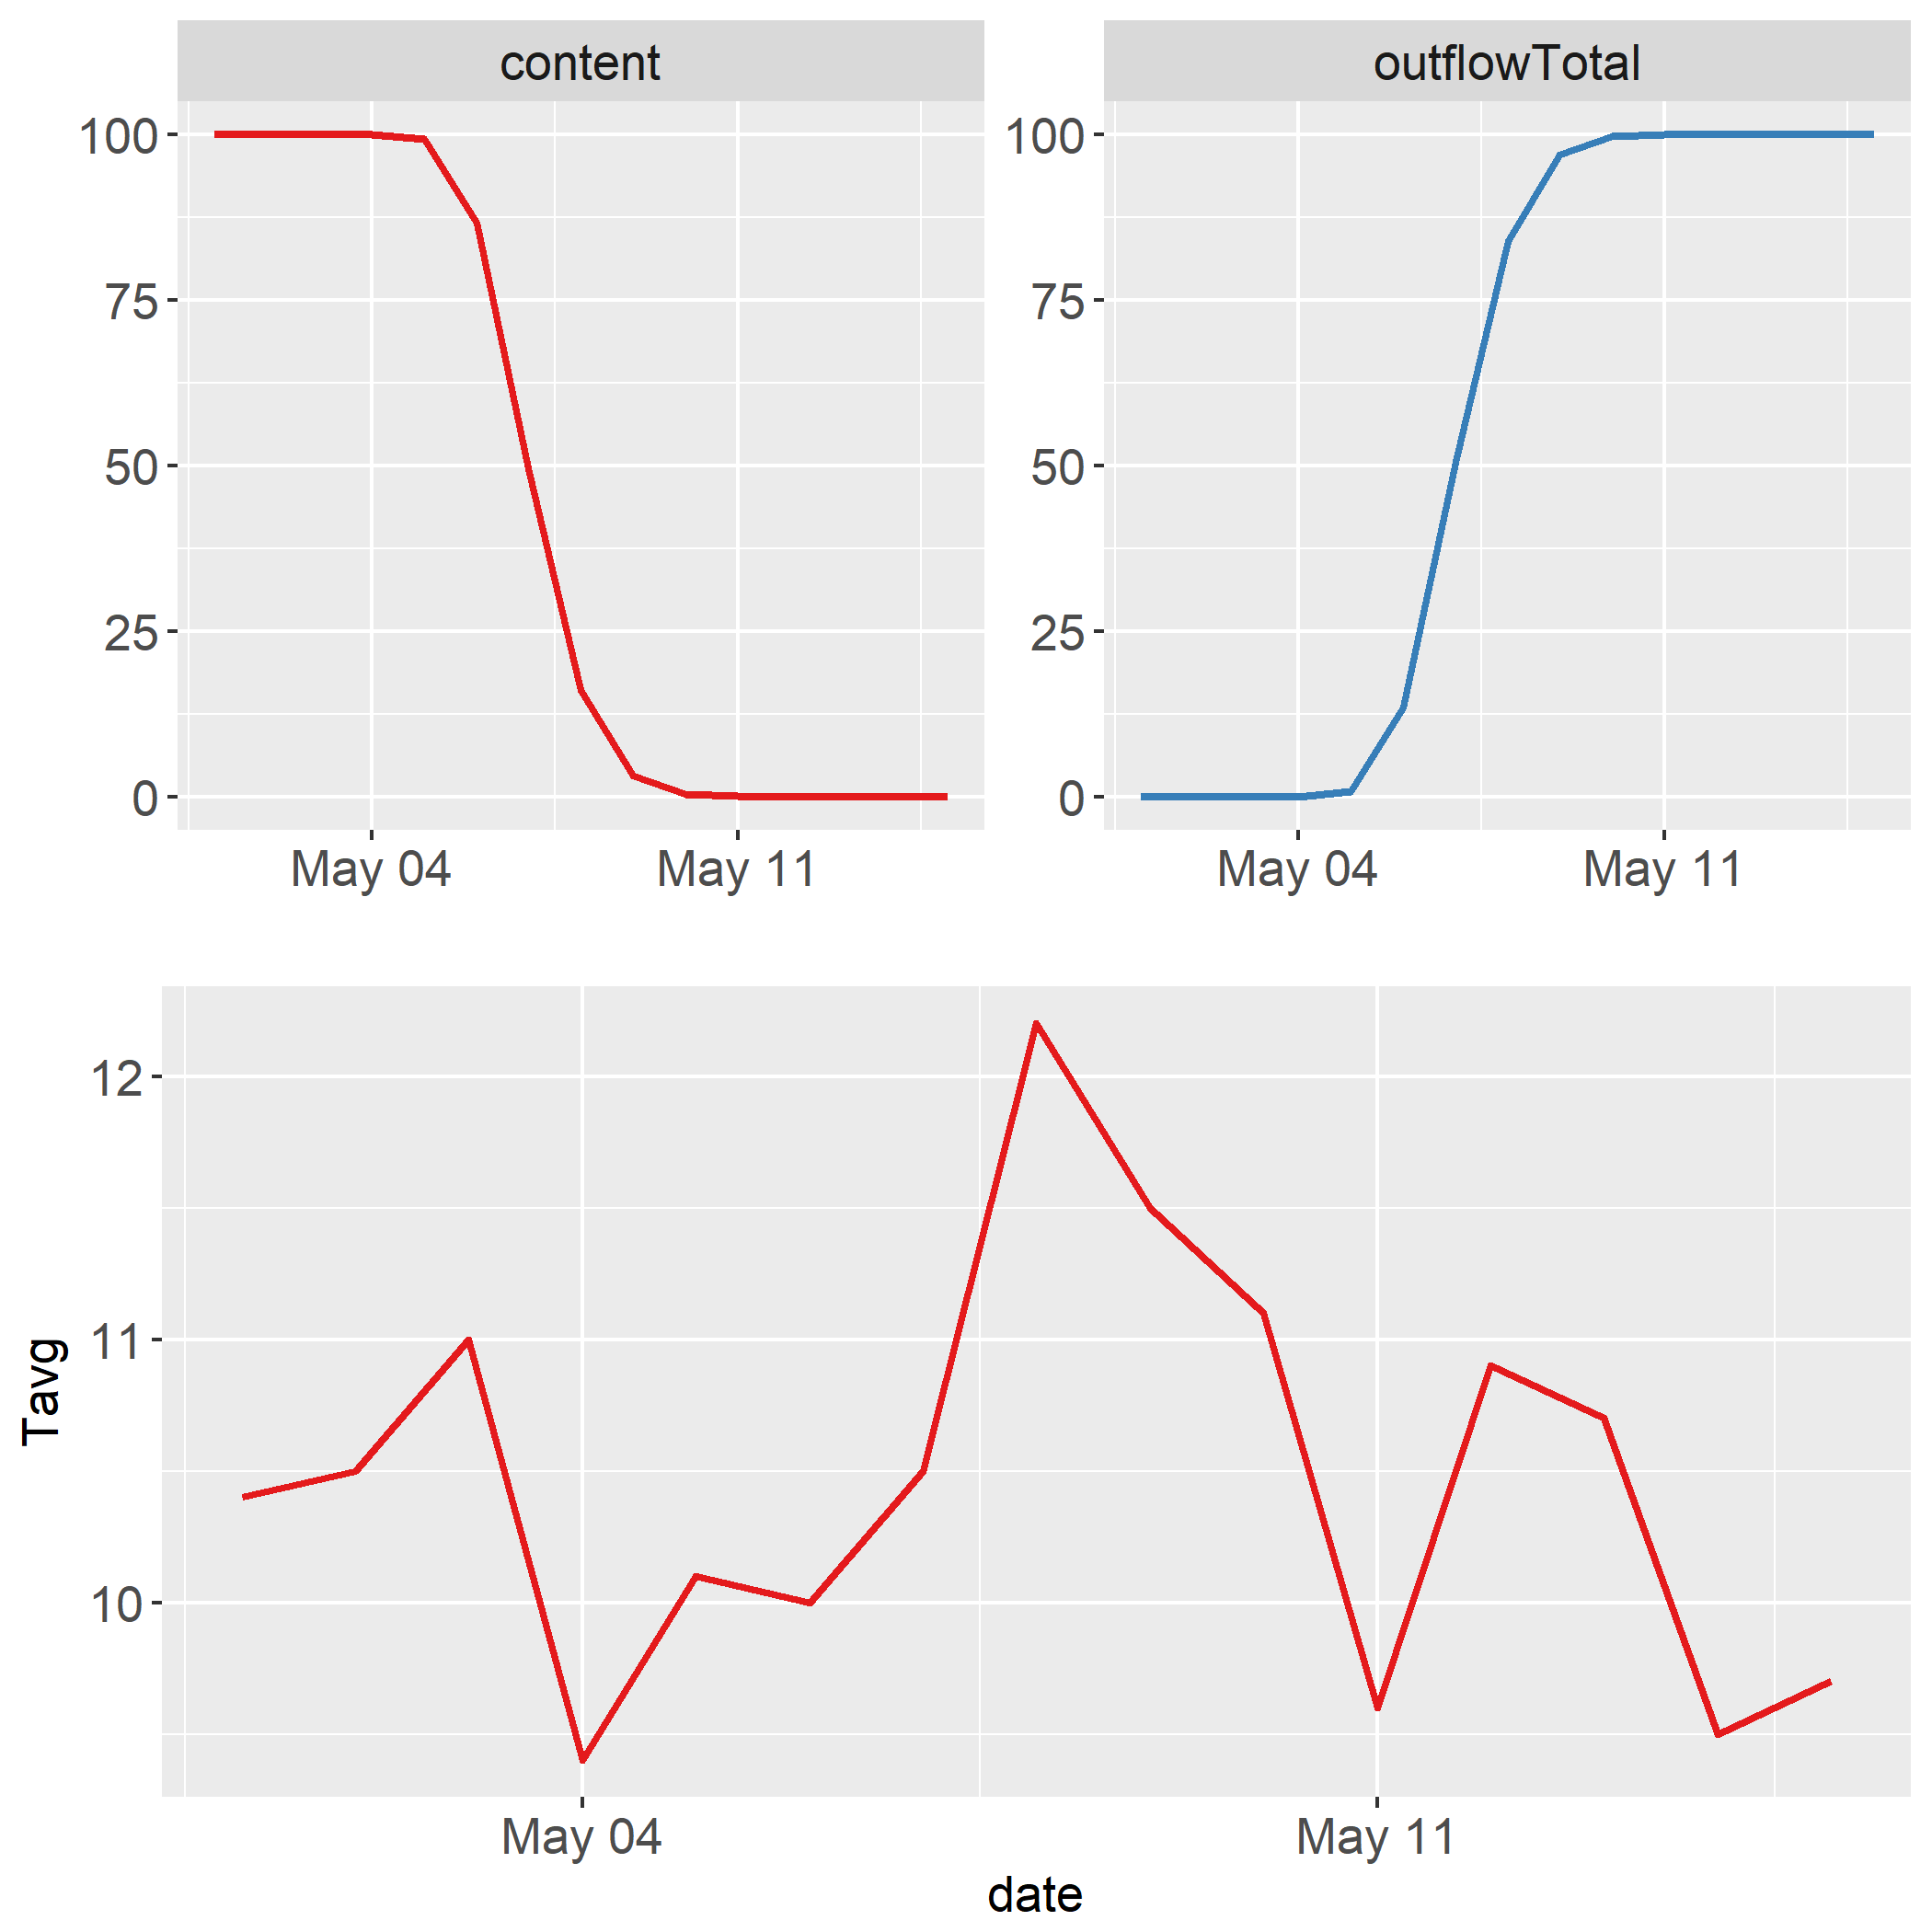
\includegraphics[scale=0.5]{graphics/egg4}
\caption{Egg hatching curves shown together with temperature records. Generated by \filename{\inputfolder/book/egg4.box}.}
\label{fig:egg4}
\end{figure}

In \filename{egg4.box} we have also added yet another \code{PlotR} output (lines 25-27) to show the daily average temperature (\code{Tavg}), which is an output port of \code{weather} named after to the column heading in the weather input file. The final outcome of the script is shown in \iref{fig:egg4}.

How did we synchronize the reading of the weather file (which begins 1 January 2009) with the calendar (which begins 1 May 2009)? This synchronization occurs automatically. Try asking for help on the \code{Records} class at the \US\ prompt:

\begin{usdialog}
> help Records
:
.calendarDateTime| |Defaults to %calendar[dateTime]%
:
>
\end{usdialog}

By default \code{calendarDateTime} refers to the \code{dateTime} port of an object named \code{calendar}. Hence the \code{calendarDateTime} port of a \code{Records} box will always hold the current date and time, as produced by the \code{dateTime} output of the \code{Calendar} object.

Should \code{calendarDateTime} fall outside of the range covered by the input file, \code{Records} will extrapolate the first record in the file to all earlier date-times and the last record in the file to all later date-times.

The box script above will output the daily average temperature of the first two weeks of May, but we missed to apply this information to drive a day-degree model for egg development. We will turn to this next, making the following alterations to the box script:
\begin{itemize}
\item Add a \code{DayDegree} model as a child of the \code{egg} model.
\item Change \code{timeStep} of the \code{egg} model to use the daily increment in day-degrees, calculated by the \code{DayDegree} model (the default \code{timeStep} is 1).
\item Change \code{duration} of the \code{egg} model to reflect a day-degree sum.
\item Increase the number of simulation \code{steps} to simulate the full egg development period.
\end{itemize}
This is how it looks:

\lstset{numbers=left}
\begin{boxscript}[label=egg05-box]
// egg5.box
Simulation sim {
  .steps = 60
  Calendar calendar {
    .timeStep = 1
    .timeUnit = "d"
    .initialDateTime = 1/5/2009
  }
  Records weather {
    .fileName = "weather/flakkebjerg 2009.txt"
  }
  Stage egg {
    .timeStep = ./time[step]
    .initial = 100 
    .duration = 140
    DayDegrees time {
      .T = weather[Tavg]
      .T0 = 8.3
      .Topt = 29
      .Tmax = 35
    }
  }
  OutputR {
    PageR {
:
:
      .xAxis = calendar[date]
      PlotR {
        .ports = (egg[content] egg[outflowTotal])   
        .ncol = 2
      }
      PlotR {
        .ports = (weather[Tavg] egg/time[total])   
        .ncol = 2
      }
    }
  }
}\end{boxscript}
\lstset{numbers=none}

The \concept{box computation model} (\iref{ch:computations}) ensures that boxes are always handled in order from top to bottom, and that any child model is handled before its parent. In this case, this means that the \code{time} model inside \code{egg} will be updated before \code{egg} itself. Thus the \code{timeStep} of \code{egg} will always get the most recent value from the \code{DayDegree} model.

As our box scripts now are getting more complicated, it is time to note that inside a box, all its inputs must be declared before any child boxes. 

In the output (\iref{fig:egg5}) you will notice that half of the eggs had hatched at the time, when around 140 day-degress had accumulated. You may wonder what induces the spread around the average. The spread is set by the \code{k} input port of \code{Stage} (\code{k} is an integer input with a default value of 30). The larger the \code{k}, the smaller the spread. 

The \code{Stage} model implements the \concept{distributed delay} algorithm of which \(k\) is the dispersion parameter (see \iref{ch:physiological-development-stage}). Note that even though the distributed-delay model introduces a spread, it is a deterministic model. Thus every run with the \code{Stage} model will give the same result, unless stochasticity is introduced elsewhere in the box script.

\begin{figure} [t]
\centering
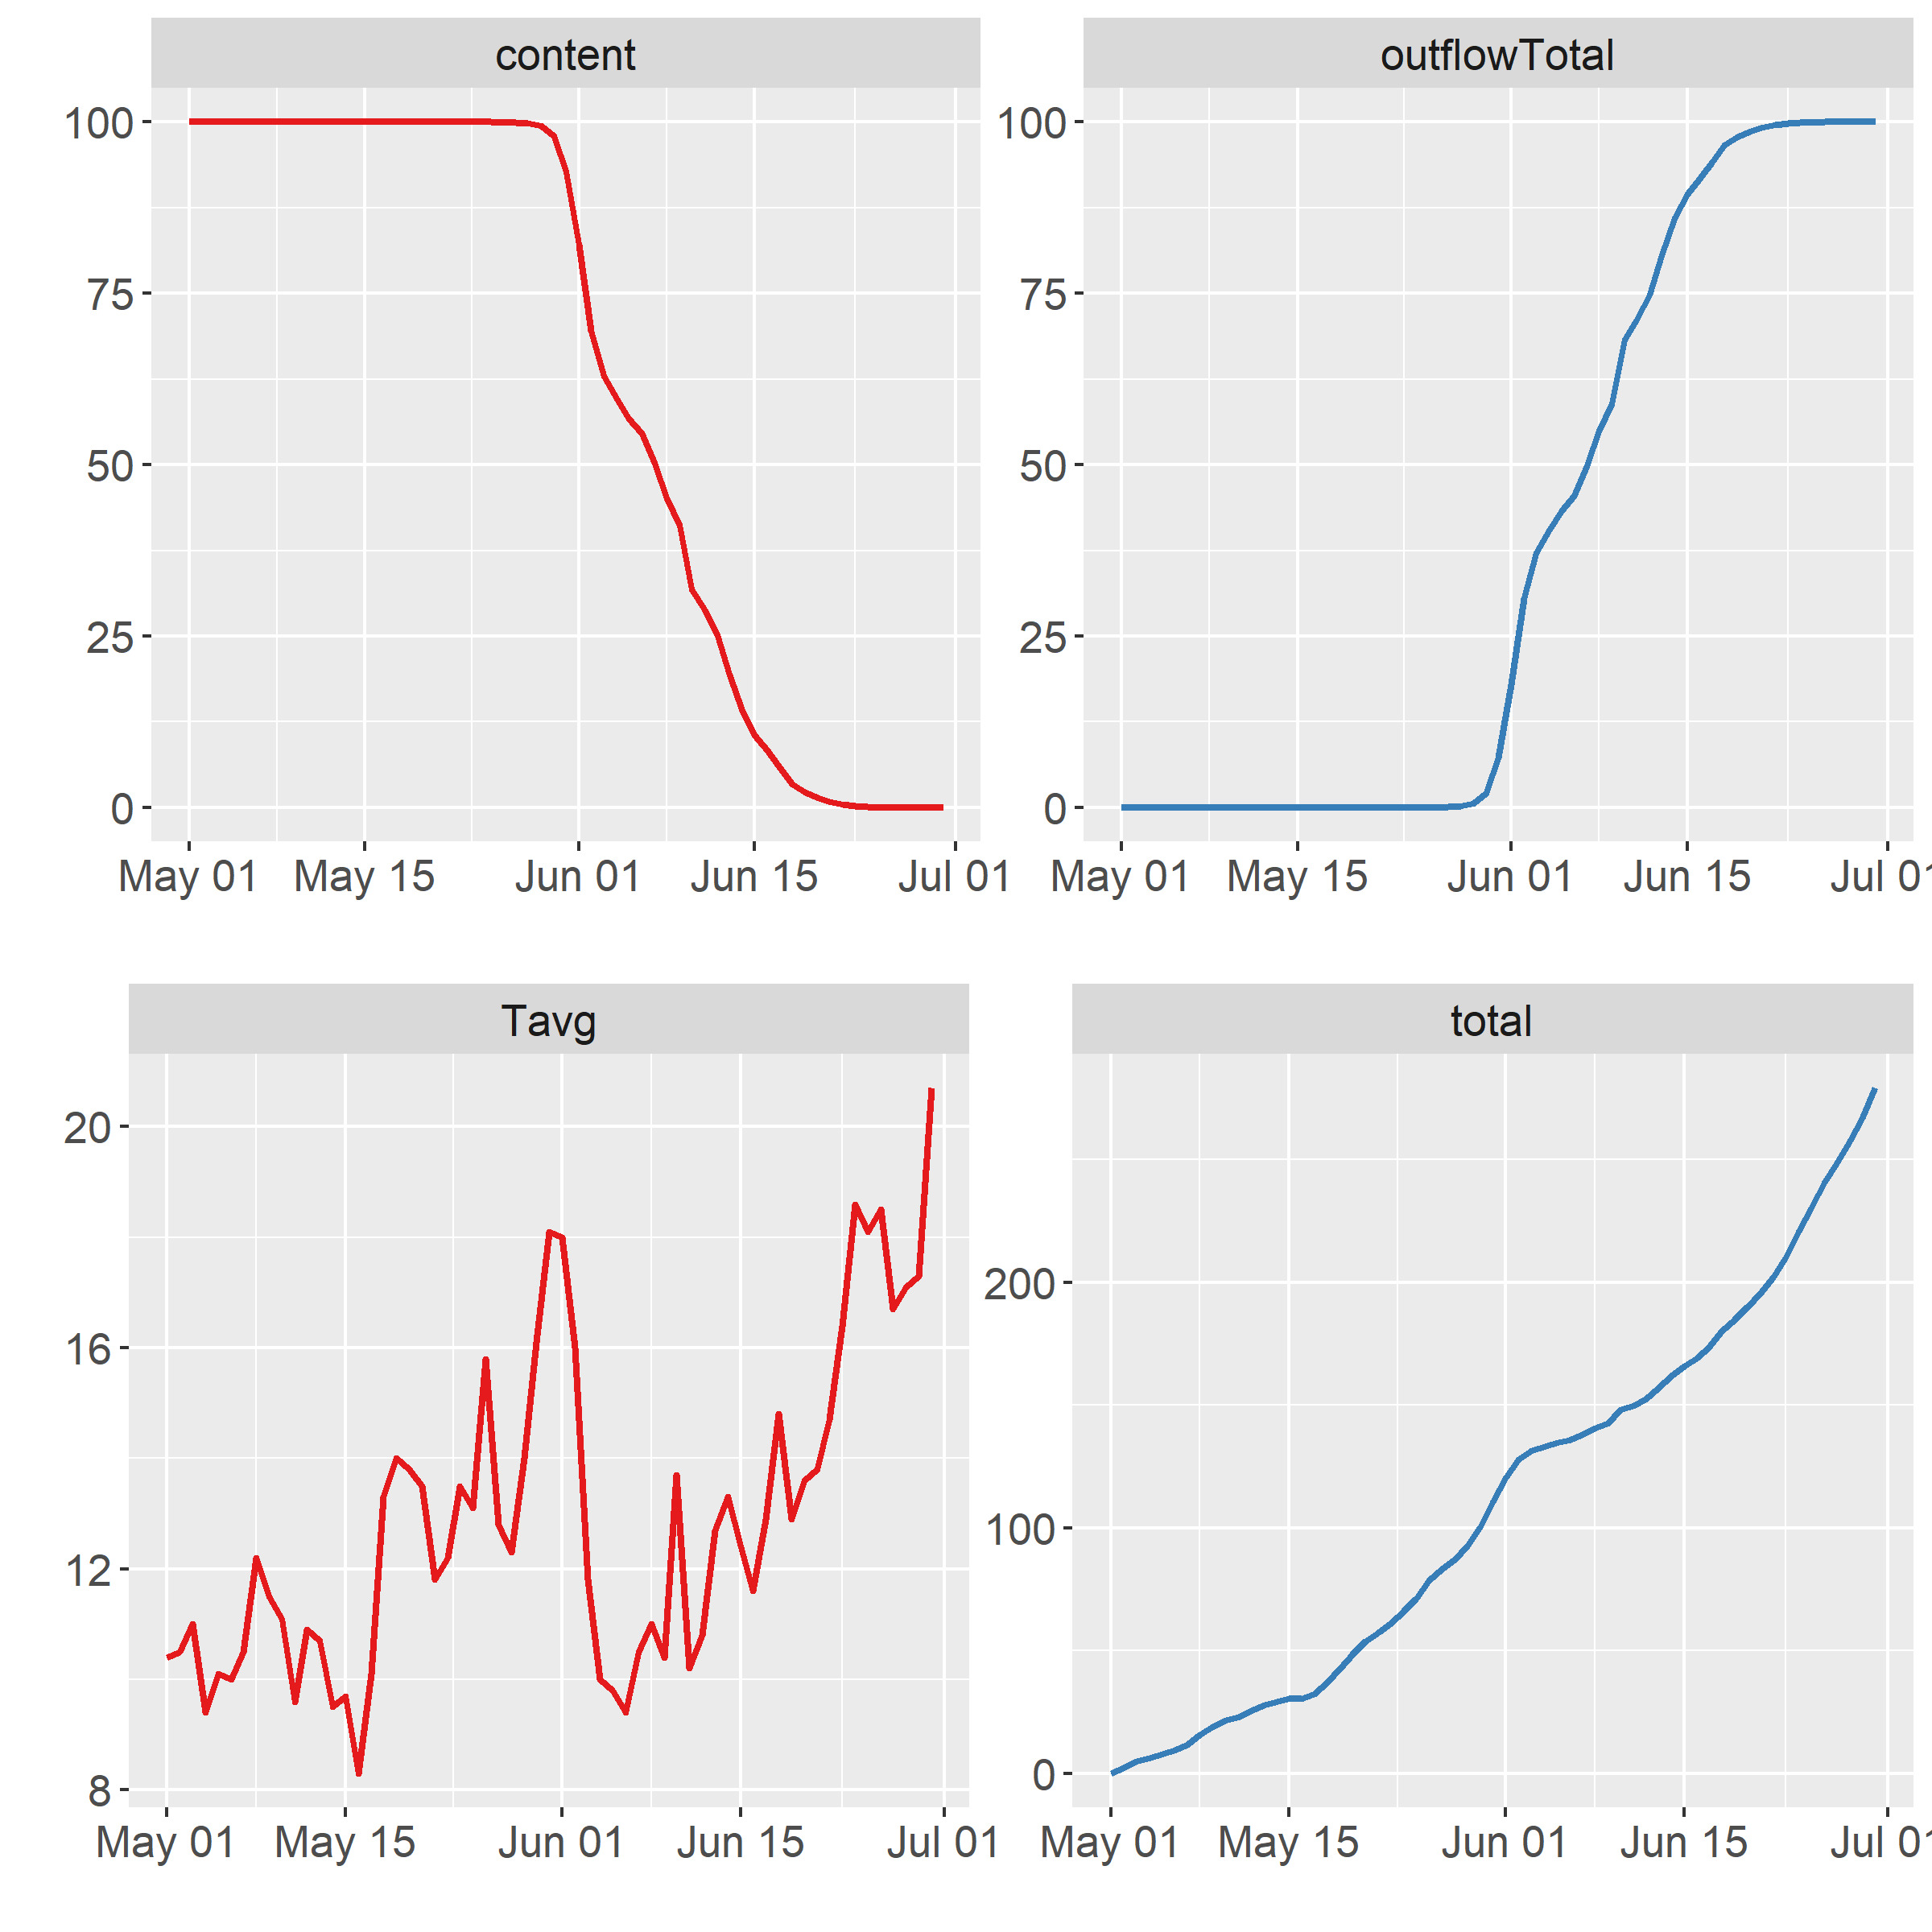
\includegraphics[scale=0.5]{graphics/egg5}
\caption{Egg hatching curves running on a day-degree scale. Generated by \filename{\inputfolder/book/egg5.box}.}
\label{fig:egg5}
\end{figure}


\section{Where do I put my own box scripts?}
\label{ch:where-box-scripts}
All the box scripts presented in this book are located in the \filename{\inputfolder/book} folder. The default location for this is in the \filename{\ushome/input} folder (see \iref{commands:set-folder}).

There are three different locations where you could place a folder for your own box scripts. That is determined by where you put your \ushome\ folder:
\begin{enumerate}
\item In the default location \ushome
\item In the developer location \devhomefolderexplained
\item In any other location, \eg\ \filename{C:/users/joe/documents/models}
\end{enumerate}

Option 1 works immediately. You just need to find the \ushome\ folder on your computer. An easy method is to load a script from this book, then edit it and then choose 'Save as...' in the editor. This will guide you to the \ushome\ folder. The drawback of option 1 is that if you upgrade \US\ to a newer version then the existing \ushome\ folder will be reconfigured (as described for the \code{reconfigure} command in \iref{commands:reconfigure}). In effect, the old \ushome\ folder will be backed up, including the folders you may have added. To re-establish your folders, you must then copy them from the backup to the new \ushome\ folder.

Option 2 will be an option only later on, when you have installed the source code package for \US. It makes sense to use that option because then you will have all your source code and box scripts in one place. However, it has the drawback that when you upgrade the \US\ source code to a newer version, you will need to move your box scripts to that newer version.

Option 3 has neither of the drawbacks above. You can keep your box scripts in the same location irrespective of any upgrades of \US. However, since the \filename{book} folder (containing all the box scripts for this book) will not be found inside your own folder, you can no longer immediately run the box scripts found in this book with this option. You will need to swap between different work folders:

For each of the options above, you can set the \ushome\ folder with the corresponding command (\cf\ \iref{commands:set-folder}):
\begin{enumerate}
\item \codenobox{set folder work HOME}
\item \codenobox{set folder work DEV}
\item \codenobox{set folder work C:/users/joe/documents/models}.
\end{enumerate}

Let's say you chose option 3 for the location of your \ushome\ folder, and that you evoked command 3 above to achieve that. Then if you wanted to study a script from this book, you should first evoke command 1. This again gives you access to all the book scripts. When your book studies are finished, you return to your own place by evoking command 3.

I suggest you stick to the default of putting your scripts inside a sub-folder of \ushome\ named \filename{input}, \eg\ in \filename{C:/users/joe/documents/models/input}. It is a good idea to keep all your box scripts neatly organized in a folder structure, together with the input files that your box scripts may rely on, such as weather and scenario files and R scripts. For this purpose, create sub-folders inside your input folder \inputfolder (\iref{fig:layout-input-folder}).

\begin {figure} [ht]
\centering
\tikzstyle{every node}=[draw=black,anchor=west]
\begin{tikzpicture}[%
  grow via three points={one child at (0.5,-0.7) and
  two children at (0.5,-0.7) and (0.5,-1.4)},
  edge from parent path={(\tikzparentnode.south) |- (\tikzchildnode.west)}]
  \node {\ushome}
   child {node {input \inputfolder}
     child {node {\textcolor{red}{ant}}
      child {node {\textcolor{red}{scenarios}}}
     }
     child [missing] {}
     child {node {book}
      child {node {scenarios}}
     }
     child [missing] {}
     child {node {papers}}
     child {node {\textcolor{red}{lion}}}
     child {node {scripts}}
   }
   child [missing] {}
   child [missing] {}
   child [missing] {}
   child [missing] {}
   child [missing] {}
   child [missing] {}
   child [missing] {}
   child {node {output \outputfolder}}
 ;
\end{tikzpicture}
\caption{A possible layout of your input folder (\inputfolder) located in \filename{\ushome/input} when working with option 1 or 2 (see text). Folder names in red have been added to the default hierarchy of folders with names in black.}
\label{fig:layout-input-folder}
\end{figure}

In this example, you have added the \filename{ant} and \filename{lion} folders to hold box scripts for two different modelling projects. Moreover, you have put a \filename{scenarios} sub-folder inside \filename{ant}.

If you have downloaded the \US\ source code package, you will find a copy of the \filename{\ushome/input} folder in the \filename{\devhome/input} folder. This is the original location of the input files packed into the \US\ installer file. It is all right for you to put your box scripts inside the \filename{\devhome/input} folder. That's option 2 above.

